\documentclass[letterpaper]{article}

% NIPS header
\usepackage{nips10submit_e,times} 
\usepackage{helvet} 
\usepackage{courier}
\usepackage{url}

% fancy symbols
\usepackage{amsmath}
\usepackage{amsthm}
\usepackage{amssymb}
% \usepackage{natbib}
\usepackage{graphicx}

\newtheorem{thm}{Theorem}
\newtheorem{lemma}{Lemma}
\newtheorem{definition}{Definition}
\newtheorem{question}{Question}

\title{Classifying reviews}
\author{Ertan Dogrultan, Cesar Romero, Paul Wais\\
Computer Science Department \\
University of California, Los Angeles\\
Los Angeles, California 90095\\
\texttt{\{ertan,romero\}@cs.ucla.edu, pwais@ucla.edu}}

\nipsfinalcopy

\begin{document}
\maketitle
\begin{abstract}
In this project, we study the learning task of predicting ``usefulness''
votes of product and business reviews.  We have obtained 2 million
Amazon reviews and 15,000 Yelp reviews annotated with voting
information.  We wish to predict whether a review will achieve a high
ranking on the scoreboard of reviews voted ``useful''.  In particular,
we consider a binary labeling task where we assign a positive
``usefulness'' label to a review if its positive vote count falls at or
above the pth percentile of all vote counts (and assign a negative
label otherwise).  To predict these labels, we have implemented about
two dozen textual and contextual features inspired by Pang et al. \cite{PangSentimentClassification}
\end{abstract}

\section{Introduction}
\label{sec:introduction}

We tell a story to motivate the problem. We mention Jenn's
work~\cite{JennLearnDiffDomains} and the sentiment classification
work~\cite{PangSentimentClassification}.

\section{Feature Extraction and Labelling the Data}
We have divided the features into several categories.
\subsection{Features}
\label{sec:features}
\subsubsection{Word Frequencies and Counts}
Our simplest feature is the number of words in the review. Similarly,
we calculate the average number of words per sentence and
total number of sentences in the review. Furthermore, we count the
number of URLs.

We obtain many different sets of words divided with respect to their
contextual meanings i.e. time, space, comparison, contrast, summary,
suggestion, emphasis, etc. and we count the number of occurences of
these in a review. For instance, comparison words are
\emph{similarly, likewise,} etc., contrast words are \emph{but,
  however, nevertheless, in spite of,} etc. Moreover, we have some
other sets of special words such as SAT, GRE lists on which we apply the same procedure.  We normalize by dividing each of them by the total
number of words in the body of the review and use them as features.   

\subsubsection{Sentential Errors}
We count the grammar and spelling errors with libraries using
Microsoft Word. In addition to those, we get the number of
capitalization mistakes and words with all capital letters. Similarly, we
divide those count by the total number of words in the review to have
a better sense of measurement.  

\subsubsection{Scores}

\subsubsection{Product/Service Related Features} 
This feature is somewhat different than the previous ones
because it depends on the product as opposed to a particular
review. We include the price of the product from the Amazon data set and
discretize it so that we have a corresponding measurement of price
range as we have in Yelp reviews (an integer between 1-4). 

\subsection{Deciding on the Labelling}
In the early experiments, we used $50^{th}$ percentile cutoff to label the
review as useful. In other words, if the positive votes for a review is above
$50^{th}$ percentile, we labeled it as useful. However, this approach affected our classification
accuracy. Therefore, we pushed the thresholds to more extreme values
to get rid of the noisy data in the middle. Currently, we label a review as useful
if its positive votes are in the $75^{th}$ percentile or above and not
useful if they are 
in the $5^{th}$ percentile or below. We observe the reflection of this
approach on the confusion matrices. We will discuss more about this in
Section \ref{sec:single_domain}.


\section{Single Domain Experiments}
\label{sec:single_domain}  
We run the experiments using Support Vector Machines, AdaBoost and
Naive Bayes with two different feature configurations. In the first
configuration, we have different sets of words as we described in
Section \ref{sec:features}. We compute the frequencies of those
words and use each calculated frequency as a single feature. We call
this feature encoding, dense. 

Our second feature encoding approach aims to generate more weak classifiers out of the sets
of words. We assume every single word from these sets is a feature and
we get the corresponding weak classifier by computing their
frequencies. We call this feature encoding, sparse. The main
motivation behind this approach is increasing the dimension for
classification which can be useful for SVMs and AdaBoost algorithms.

\begin{table}[ht]
\centering
\begin{tabular}{c | c c | c c}
 & \multicolumn{2}{|c|}{Amazon} & \multicolumn{2}{|c}{Yelp} \\
\hline
Algorithm & Training Err. & Cross Val.(5 fold) & Training Err. & Cross Val.(5 fold)\\
\hline
SVM (Linear) 		& $71.0316\%$ & $70.8\%$ & $70.305\%$ & $70.2879\%$\\
SVM (Polynomial) 	& $73.1041\%$ & $72.4316\%$ & --- & 71.3417\%\\
SVM (Gaussian) 		& $66.053\%$ & $66.053\%$ & $68.7971\%$ & $69.1484\%$\\
AdaBoost 			& $71.0316\%$ & $72.201\%$ & $71.3588\%$ & $70.3136\%$\\ 
Naive Bayes 		& $70.719\%$ & $70.6727\%$ & $66.9037\%$ & $66.5781\%$\\ 
\end{tabular}
\caption{Accuracy results using dense feature encoding}
\label{tab:dense}
\end{table}


\begin{table}[ht]
\centering
\begin{tabular}{c | c c | c c}
 & \multicolumn{2}{|c|}{Amazon} & \multicolumn{2}{|c}{Yelp} \\
\hline
Algorithm & Training Err. & Cross Val.(5 fold) & Training Err. & Cross Val.(5 fold)\\
\hline
SVM (Linear) 		& --- & $72.2357\%$ 		& --- & $70.0163\%$\\
SVM (Polynomial) 	& --- & $66.053\%$ 		& --- & $70.0592\%$\\
SVM (Gaussian) 		& --- & $72.4673\%$ 		& --- & $71.1062\%$\\
AdaBoost 			& $71.68\%$   & $70.7769\%$ & $71.2091\%$ & $70.7286\%$\\ 
Naive Bayes 		& $76.8091\%$ & $73.0346\%$ & $77.1733\%$ & $67.9567\%$\\ 
\end{tabular}
\caption{Accuracy results using sparse feature encoding}
\label{tab:sparse}
\end{table}

Before we get into the details about SVMs and AdaBoost, we would like
to state some facts about the Naive Bayes classifier and its
significant performance improvement when we switch to sparse feature
encoding. As we stated in the progress report the main problem with
this classifier is claimed to be the lack of low entropy feature
distributions \cite{naivebayes}. We pointed that the unrealistic
assumption of conditional independence between the features hurts the classification
significantly which is the nature of dense feature encoding. There are
some overlaps in the contextual meaning of those lists as well as
common words. Therefore, we remove this dependency factor
when we use sparse encoding and as you can see from Tables
\ref{tab:dense} and \ref{tab:sparse}, the training accuracy of
the Naive Bayes classifier increases from $70.719\%$ to $76.8091$ for
Amazon data set and from $66.9037\%$ to $77.1733$ for Yelp data set.  

Looking at the accuracies of AdaBoost algorithm and linear SVM in
dense and sparse configurations, we observe similar accuracies for
both Amazon and Yelp data set. One of the main
reasons is the class distribution (the choice of percentile to
label the sample as useful) has a significant
effect on the accuracy. This conclusion originates from the
observation of ``bad'' confusion matrices for the classifiers. 

\section{Questions}
Ertan: can we estimate $\gamma$ from the training error of each classifier from the AdaBoost standard out?  If $\gamma$ is large, then perhaps that might expect why AdaBoost didn't do much better than the other classifiers.  

Guys, so it looks like the Amazon and Yelp data sets have almost identical distributions.

\begin{figure*}[h]
	\centering
	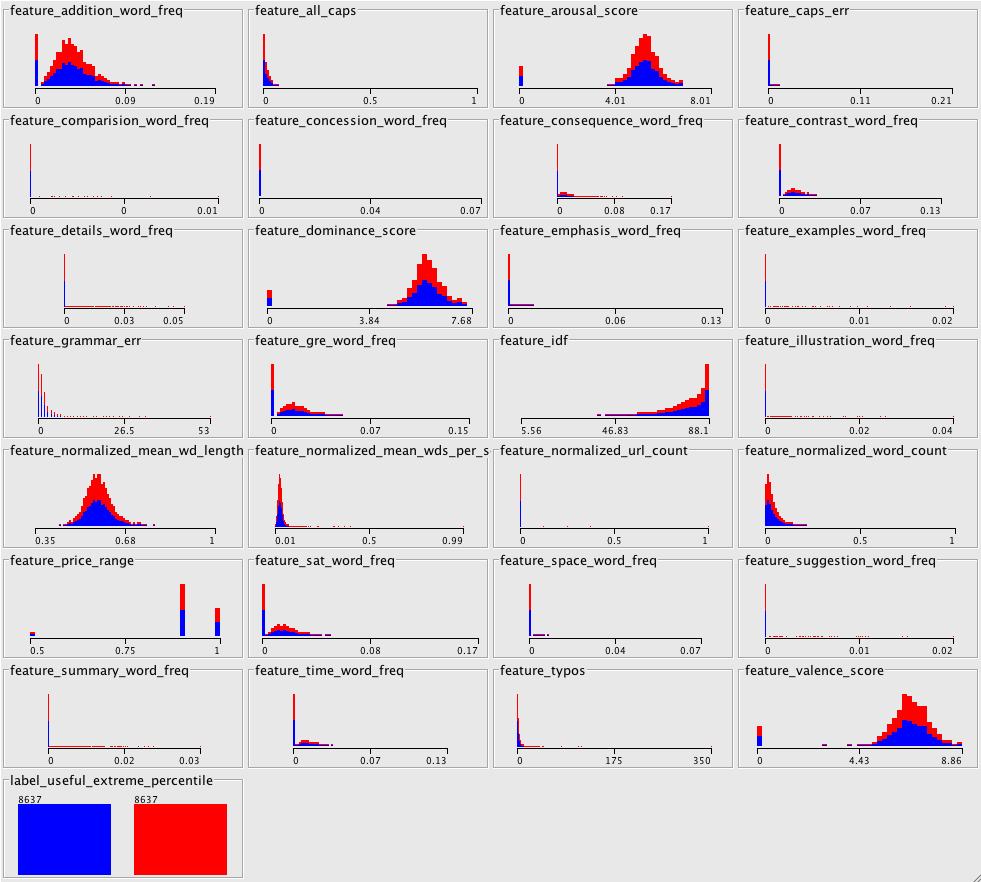
\includegraphics[width=0.5\linewidth]{adaptation_unlabeled_features}
	\caption{Feature distributions for the unlabeled data sets $U_{\textrm{A}}$ and $U_{\textrm{Y}}$.  
	Blue indicates Amazon data feature values and red indicates Yelp feature values.}
\end{figure*}

I tried running the SVM again on our data set and it got 50\% accuracy... perhaps when a data set is not separable at all an SVM picks hyperplanes that just split the data in half... in any case, I think our distance $\zeta(U_{\textrm{A}}, U_{\textrm{Y}})$ should actually be more like 0?

\section{Domain Adaptation}
\label{sec:background}

\emph{Here, we explain what domain adaptation is and its important
prameters.}
We are interested in being able to classify reviews in general - not
just from a specific source or category. A natural problem to consider
is Domain Adaptation. In this setting, there is a source domain $S$
and a target domain $T$. The goal is to be able to classify reviews in
$T$ when most of our data comes from $S$. 

Include the fancy Theorem here that will be used to predict the error
of the calssifiers in the domain adaptation setting.

\subsection{$\alpha$-error}
\label{sec:alpha-error}

Explain the $\alpha$-error here.

\subsection{Estimating the distance}
\label{sec:estimating-distance}

We train a linear classifier to learn to which domain a review
belongs. The error of this classifier is used as an estimate of the
distance between the distributions.

\section{Mid-quarter report}
\label{sec:mid-quarter-report}

In the report we cited~\cite{citeulike:352583} among others. Figure~

\begin{figure*}[h]
  \centering
  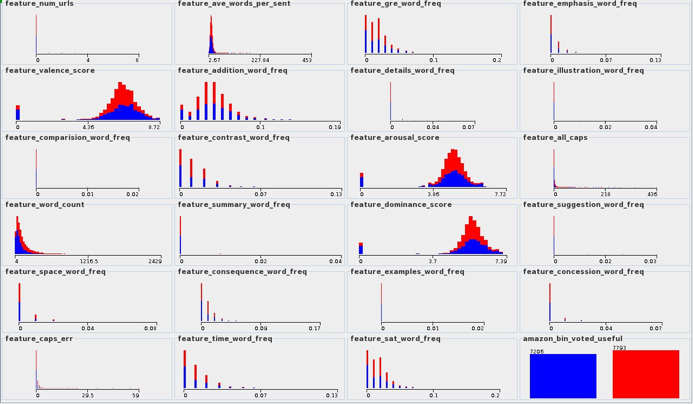
\includegraphics[scale=.5]{features_distributions}
  \caption{This is the figure from the report}
  \label{fig:dist}
\end{figure*}

\section{Features}
\label{sec:features}

A concise and example-driven description of all our features.  This
will probably take a little while to write :). And we should probably
have a reference to ANEW~\cite{DoddsANEWPaper}.

Link to our github:
\url{https://github.com/pwais/thumbsup}

\section{Experiments}
\label{sec:experiments}

We present two sets of experiments. In the first set, we use different
models to learn the quality of the review using the features described
in~\ref{sec:features}. Then, we use the model that performs best in
the first set of experiments to classify reviews in a domain
adaptation setting. We use the WEKA machine learning suite for our
experiments~\cite{weka}.

\subsection{Learning Reviews}
\label{sec:learning-reviews}

We use three different models to learn the quality of the reviews:
Support Vector MAchines (SVMs), AdaBoost, and Naive Bayes.

\emph{Our original data includes a lot of noise. We can probably talk
  here about taking only the extreme cases: either very good (over
  85th percentile) or very bad (under 5th percentile).}

\subsection{Domain Adaptation}
\label{sec:domain-adaptation}

In this set of experiments we use the \emph{insert model here} to
learn from both domains. For this experiments, Yelp is considered to be
the \emph{target} and Amazon the \emph{source}.

We estimate the distance between the distributions, $\zeta$ , using the metod
previously explained in the domain adaptation Section. For the first
set of domain adaptation experimentes, we vary the value of $\beta \in
\{0.1, 0.2, 0.4, 0.8\}$ while holding $\zeta$ constant.

Using a fixed $\beta$ we want see how well the classifier performs
when the distance between the target and source distribution
varies. To alter $\zeta$, we consider only a specific category on each
domain. From the source domain (Amazon), we consider the set of
categories $C_S=\{$ Books, Electronics, DVDs and Clothing\}. From the
target domain (Yelp) we consider only one category
$C_T=$\{Restaurants\}. For each combination in $C_s\times C_T$ we train
and test a different classifier. Notice that, to estimate the distance
between any of the two categories in the four possible combinations,
we need to train a separate linear classifier to estimate the distance
as we did before. Figure~\ref{fig:domain-adaptation} shows the errors
of these classifiers together with their theoretical bounds.

\begin{figure}
  \centering
  
  \caption{Domain Adaptation Experiments}
  \label{fig:domain-adaptation}
\end{figure}

\section{Citations to use}
Jenn's domain adaption paper \cite{JennLearnDiffDomains}\\
ANEW paper \cite{DoddsANEWPaper}\\
Pang et al sentiment classification \cite{PangSentimentClassification}\\
The WEKA paper that they ask users to cite \cite{weka} \\
Naive Bayes paper \cite{naivebayes}
\bibliographystyle{IEEEtran}
\bibliography{IEEEabrv,bib}

\end{document}
